\section{Configuración de Postgresql}

Los archivos utilizados para configurar postgresql son tres: \cite{Obe2012}

\begin{itemize}
\item \textbf{postgresql.conf}: El principal archivo de configuración de postgresql, controla configuraciones generales como la cantidad de memoria RAM a utilizar, la localización física de las bases de datos, las ips a las que escucha postgresql, la configuración de los logs, etc.
\item \textbf{pg\_hba.conf}: controla la seguridad, gestiona el acceso al servidor indicando que usuarios pueden acceder a que BD, que Ips o grupos de Ips están permitidos de conectarse y el esquema de autenticación esperado.
\item \textbf{pg\_ident.conf}: Es el archivo que mapea los usuarios del SO con los usuarios del servidor
\end{itemize}

Para conocer donde están localizados en el sistema, se puede utilizar un superusuario del servidor para ejecutar la siguiente consulta:\\

\textbf{\$ sudo su postgres -c ``psql -d Bd\_prueba''}\\

Y luego:\\

\begin{pyglist}
SELECT name, setting
FROM pg_settings
WHERE category = 'File Locations';
\end{pyglist}


Una forma sencilla de ver las configuraciones en postgresql.conf es consultar la tabla pg\_settings, por ejemplo la siguiente consulta devuelve los valores de seis parámetros de postgresql.conf.\\

\newpage

\begin{pyglist}
 SELECT name, context, setting, boot_val, reset_val FROM pg_settings
 WHERE name
 in ('listen_addresses','max_connections','shared_buffers','effective_cache_size',
     'work_mem', 'maintenance_work_mem')
 ORDER BY context,name;
\end{pyglist}



También se puede utilizar el comando show para ver cada parámetro de configuración por separado con su valor respectivo, por ejemplo:\\

\begin{pyglist}
show maintenance_work_mem;
show work_mem;
show all;
\end{pyglist}

\section{Creando Bases de Datos}

La forma más sencilla de crear una base de datos es ingresando a un cliente (como psql) y utilizando el comando:\\

\begin{pyglist}
CREATE DATABASE mi_bd;
\end{pyglist}

El dueño de la Bd será el usuario en el sistema y la BD será una copia de template1. Es potestad del creador de una Base de Datos eliminarla posteriormente, lo cuál elimina a su vez todos sus objetos como tablas, índices, funciones, etc así tengan otros dueños.\\

La primera base de datos en ser creada al instalarse PostgreSQL es \textit{postgres} y luego \textit{template0} y \textit{template1} que son plantillas de bases de datos desde las cuáles se copian las nuevas bases en ser creadas. Todo cambio que se haga en \textit{template1} se replicará en toda nueva Base de datos, por lo que se recomienda ser muy prudente con las plantillas.\\

Si se desea crear una base de datos con otro dueño fuera del usuario que la está creando, se agrega el parámetro OWNER.\\

Por ejemplo:\\

\begin{pyglist}
CREATE DATABASE nombre_db OWNER usuario_curso;
\end{pyglist}

Solo el superusuario puede crear una base de datos para otro usuario.


\subsection{Comando createdb}

Como conveniencia se puede utilizar el comando \textit{createdb} desde la terminal:\\

\textit{createdb nombre\_db}\\

Lo que hace \textit{createdb} es conectarse a la base de datos \textit{postgres} y ejecuta \textit{CREATE DATABASE} utilizando el usuario del sistema desde el cuál se le ejecuta.\\

Mediante parámetros se puede utilizar \textit{createdb} de forma más versátil, con -O se indica el owner de base de datos creada, con -U el usuario con el se conectará a \textit{postgres} entre otros parámetros.\\

Por ejemplo:\\

\textit{createdb -U postgres -O usuario\_curso nueva\_bd}\\

Va a crear una base de datos llamada nueva\_bd mediante el usuario postgres y va a ser propiedad de usuario\_curso.

\subsection{Creando una base de datos plantilla}

Una base de datos de plantilla (Template DB) es una base de datos que sirve de plantilla para crear otras bases de datos. Se puede crear una Bd a partir de cualquier otra Bd, pero PostgreSQL permite que se definan Bds específicamente de plantilla. La principal diferencia es que una Bd definida como template no puede ser eliminada y puede ser utilizada por cualquier usuario con capacidad de crear bases de datos como plantilla para una nueva BD.\\

La principal base de datos plantilla es \textit{template1} a partir de la cual se crean todas las bases de datos en caso no se mencione otra plantilla. Si se agregan objetos a \textit{template1}, se replicarán en todas las nuevas bases que se creen teniendo a \textit{template1} como plantilla.\\

Existe una segunda plantilla, \textit{template0}, que contiene el mismo contenido inicial que \textit{template1}. A diferencia de la segunda, \textit{template0} nunca debe ser modificada, ya que al crear una base de datos tomando como plantilla \textit{template0}, se crea una base limpia de todo cambio posterior, lo cuál es especialmente valioso al restaurar un backup de pg\_dump ya que debe ser restaurado sobre una base de datos sin modificación alguna.\\

Para crear una copia de \textit{template0} se ejecuta:\\

\begin{pyglist}
CREATE DATABASE dbname TEMPLATE template0;
\end{pyglist}

O desde la terminal:\\

\textit{createdb -T template0 dbname}\\

Además de las plantillas predeterminadas, se pueden utilizar otras bases de datos como plantillas, con la limitante de que ninguna otra sesión puede estar conectada a la base de datos fuente mientras es copiada.\\

Si se ha diseñado una Bd y se quiere convertirla en una plantilla, se ejecuta el siguiente comando como superusuario:\\

\begin{pyglist}
UPDATE pg_database SET datistemplate=true WHERE datname='mi_bd';
\end{pyglist}

\subsection{Eliminar una Base de Datos}

Las bases de datos se destruyen con el comando \textit{DROP DATABASE}.\\

\begin{pyglist}
DROP DATABASE nombre_db;
\end{pyglist}

Solo el dueño de una base de datos puede eliminarla. Eliminar una Base de datos implica destruir todo su contenido y es una acción que no puede ser deshecha.\\

No se puede ejecutar el comando \textit{DROP DATABASE} mientras se está conectado a la base de datos a ser eliminada, se debe hacerconectado desde otra base de datos.\\

Existe un comando de consola, dropdb, para eliminar bases de datos.\\

\textit{dropdb nombre\_db}

\section{Creando Esquemas}

Los esquemas son una forma lógica de partir una base de datos en mini contenedores. Se pueden dividir los esquemas por funcionalidad, usuarios o cualquier otro atributo que se desee. Además de la partición lógica, proveen una forma sencilla de repartir privilegios. \\

Para crear un esquema en una BD, nos conectamos a la Bd y ejecutamos el comando:\\

\begin{pyglist}
CREATE SCHEMA mi_esquema;
\end{pyglist}

Para acceder a un objeto en un esquema se escribe el nombre del esquema seguido por el nombre ddel objeto separados por un punto.\\

\textit{schema.table}\\

Esta forma de nombrar una tabla funciona para toda aplicación, incluyendo comandos para modificar la tabla, leer y escribir datos.\\

Para crear una tabla en el nuevo esquema se debe utilizar:\\

\begin{pyglist}
CREATE TABLE mi_esquema.mitabla (...);
\end{pyglist}

La ruta por defecto (search\_path) definida en \textit{postgresql.conf} es \textbf{“\$user”, public}. Lo cual significa que si hay un esquema con el mismo nombre que el del usuario en el sistema, entonces todos los objetos van a revisar primero el esquema con el mismo nombre del usuario y luego el esquema público.\\

Los esquemas son también utilizados para abstraer los nombres de las tablas, debido a que el nombre solo debe ser único dentro del esquema y muchas aplicaciones explotan esta característica creando tablas con el mismo nombre en diferentes esquemas de tal manera que se carga una diferente dependiendo del usuario en el sistema.\\

Los esquemas sirven por ejemplo para incluir módulos externos (contrib) dentro de un esquema de tal manera que los nombres de sus objetos no puedan entrar en conflicto con el nombre de los objetos de la BD.\\

Se puede pensar en esquemas como en directorio pero sin la posibilidad de ser anidados.\\

Otra forma de asignar permisos es mediante Pgadmin3, el cuál tiene una completa interfaz para asignar permisos.\\

\begin{figure}[ht!]
   \centering
   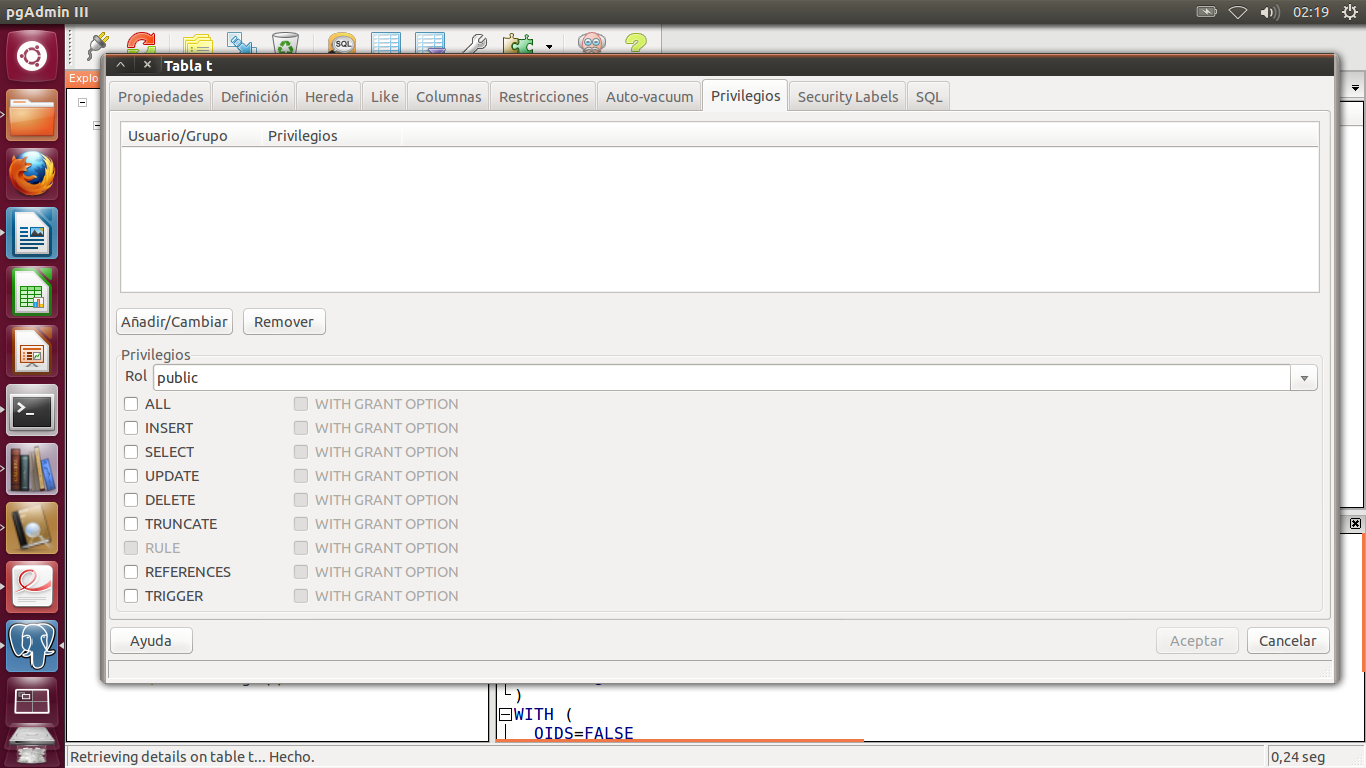
\includegraphics[scale=0.35]{imagenes/pgadmin3-privilegios.png}
   \caption{Asignación de privilegios en Pgadmin3}\label{graf:pgadmin3-privilegios}
\end{figure}

\newpage

\subsection{Permisos}

Si se quiere dar permisos a un esquema que recién se ha creado, se van a utilizar los comandos ALTER DEFAULT PRIVILEGES y GRANT.\\

Por ejemplo, para que todos los usuarios de una BD tengan acceso a EXECUTE y SELECT en todas las tablas y funciones de un esquema que se creen a partir del momento en que se ejecuten se utilizarán los siguientes comandos:\\

\begin{pyglist}
GRANT USAGE ON SCHEMA contrib TO public;
ALTER DEFAULT PRIVILEGES IN SCHEMA contrib
 GRANT SELECT, REFERENCES, TRIGGER ON TABLES
 TO public;
ALTER DEFAULT PRIVILEGES IN SCHEMA contrib
 GRANT SELECT, UPDATE ON SEQUENCES
 TO public;
ALTER DEFAULT PRIVILEGES IN SCHEMA contrib
 GRANT EXECUTE ON FUNCTIONS
TO public;
ALTER DEFAULT PRIVILEGES IN SCHEMA contrib
 GRANT USAGE ON TYPES
 TO public;
\end{pyglist}

Si el esquema ya está definido con sus tablas y funciones, se pueden dar permisos uno por uno o darle permisos a todos mediante GRANT .. ALL .. IN SCHEMA.\\

\begin{pyglist}
GRANT USAGE ON SCHEMA contrib TO public;
GRANT SELECT, REFERENCES, TRIGGER
 ON ALL TABLES IN SCHEMA contrib
 TO public;
GRANT EXECUTE ON ALL FUNCTIONS IN SCHEMA contrib TO public;
GRANT SELECT, UPDATE ON ALL SEQUENCES IN SCHEMA contrib TO public;
\end{pyglist}

Es común buscar que un esquema sea propiedad de otro usuario, para asi restringir las actividades de los usuarios a namespaces restringidos. La sintaxis es:\\

\begin{pyglist}
CREATE SCHEMA nuevo_esquema AUTHORIZATION usuario_curso;
\end{pyglist}

Los esquemas cuyo nombre empieza con \textit{pg\_} son utilizados el sistema y no se recomienda su creación por los usuarios debido a que futuras versiones de Postgresql pueden utilizar el nombre elegido.\\

Cuando no se define explícitamente un esquema, el objeto creado entra en el esquema “public”, por lo cual es igual escribir:\\

\begin{pyglist}
CREATE TABLE productos ( ... );
\end{pyglist}

Y\\

\begin{pyglist}
CREATE TABLE public.productos ( ... );
\end{pyglist}

\subsection{Eliminar esquemas}

Para eliminar un esquema este debe estar vacio (todos los objetos en su interior deben haber sido eliminados) y se utiliza:\\

\begin{pyglist}
DROP SCHEMA myschema;
\end{pyglist}

Para eliminar un esquema incluyendo todos sus objetos utilizar:\\

\begin{pyglist}
DROP SCHEMA myschema CASCADE;
\end{pyglist}

\section{Ruta de Búsqueda de Esquemas}

Los nombres completos incluyendo el del esquema son tediosos de escribir, además de que no es bueno ``hardcodear'' los nombres de los esquemas en las aplicaciones. Al llamar a las aplicaciones solo por su nombre, el sistema determina que tabla es buscando en todos los esquemas presentes. El primer objeto con el nombre indicado que encuentre es escogido como el buscado.\\

El primer esquema en la ruta de búsqueda (search path) es llamado el esquema actual (current schema), además de ser el primer esquema en la ruta de búsqueda es también el esquema por defecto donde se crearan las nuevas tablas si no se especifica un esquema en particular.\\

Para ver la actual ruta de búsqueda se utiliza:\\

\begin{pyglist}
SHOW search_path;
\end{pyglist}

Para colocar un nuevo esquema en la ruta de búsqueda:\\

\begin{pyglist}
SET search_path TO miesquema,public;
\end{pyglist}

Lo cual hará que el nuevo esquema sea el primero en la ruta de búsqueda, si queremos dejar de considerar public en la ruta de búsqueda se utiliza:\\

\begin{pyglist}
SET search_path TO miesquema;
\end{pyglist}

\subsection{Utilización de los esquemas}

Los esquemas se pueden utilizar para organizar la data de muchas formas diferentes. Algunos patrones de uso son recomendados:

\begin{itemize}
\item Si no se crean esquemas todos los usuarios acceden al esquema \textit{public}. Esta configuración es recomendada cuando hay solo un usuario o pocos usuarios cooperantes en la base de datos.
\item Se puede crear un esquema para cada usuario con su propio nombre. Si se usa esta configuración se pueden revocar los permisos de los usuarios sobre el esquema \textit{public} de tal manera que solo puedan utilizan sus propios esquemas.
\item Para instalar aplicaciones compartidas es recomendable colocarlas en sus propios esquemas y dar permisos a todos los usuarios para acceder a ese esquema. Los usuarios pueden referirse a los objetos agregados por su nombre completo o agregar el nuevo esquema en la ruta de búsqueda.
\end{itemize}

\section{Roles}

En PostgreSQL solo existe un tipo de cuenta y es la de rol. Si el rol puede ingresar a la BD, es un usuario. Los roles puede ser parte de otros roles y cuando un rol tiene miembros, es llamado un grupo. \\

Los roles pueden ser dueños de objetos en las bases de datos (tablas por ejemplo) y pueden asignar privilegios a otros roles en esos objetos para controlar quien accede. Además, es posible hacer a un rol miembro de otros roles de tal manera que utilice sus privilegios.\\

Los roles de PostgreSQL no son iguales a los usuarios del sistema operativo, en la práctica puede ser útill mantener la correspondencia entre ambos pero no es necesario.\\

Para crear un rol se utiliza \textit{CREATE ROLE}:\\

\begin{pyglist}
CREATE ROLE name;
\end{pyglist}

Y para eliminarlo se usa DROP ROLE:\\

\begin{pyglist}
DROP ROLE name;
\end{pyglist}

Para saber que roles han sido creados utilizar:\\

\begin{pyglist}
SELECT rolname FROM pg_roles;
\end{pyglist}

O el comando \textit{{$\backslash$}du}.

\subsection{Crear un usuario}

Al terminar de instalar el gestor de Bds, se crea por defecto una cuenta llamada postgres con una base de datos llamada postgres. Antes de hacer nada, se debe entrar con este usuario mediante psql o pgadmin y crear otros usuarios. La diferencia entre un rol y un usuario es que el usuario es creado con el atributo LOGIN que le permite ingresar a una base de dato. \\

\textbf{\$  sudo su postgres -c ``psql -d postgres''}

Mediante este comando SQL se crea un usuario con capacidad de crear bases de datos.\\

\begin{pyglist}
CREATE ROLE leo LOGIN PASSWORD 'qwerty' CREATEDB VALID UNTIL 'infinity';
\end{pyglist}

Infinity es una opción por defecto por lo que no necesita ser considerada. Se puede incluir una fecha  en la cual se espera que la cuenta desaparezca.\\

Con otro comando SQL se crea un super usuario pero con un tiempo de vida limitado. Solo se puede crear un superusuario siendo un superusuario.\\

\begin{pyglist}
CREATE ROLE regina LOGIN PASSWORD '123456' SUPERUSER VALID UNTIL '2020-10-20 23:00';
\end{pyglist}

\subsection{Atributos de los roles}

Un rol puede tener diversos atributos que definan sus privilegios.\\

\begin{itemize}
\item Login: solo los roles que tienen el atributo LOGIN pueden ser utilizados como el nombre inicial a utilizar en una conexión a una base de datos. 
\item Superuser: Un superusuario de una base de datos pasa por encima de toda restricción excepto al ingresar al sistema. Es un privilegio peligroso y debe ser otorgado con mucho cuidado. Para crear un nuevo superusuario utilizar: \textit{CREATE ROLE name SUPERUSER}. Solo un superusuario puede crear otro superusuario.
\item database creation: A un rol se le debe dar de forma explícita el permiso para crear bases de datos. Para lograrlo se utiliza \textit{CREATE ROLE name CREATEDB}.
\item role creation: Para que un rol pueda crear otros roles se utiliza \textit{CREATE ROLE name CREATEROLE}.
\item initiating replication: Para que un rol pueda iniciar una replicación se debe dar permisos de replicación de login \textit{CREATE ROLE name REPLICATION LOGIN}. 
\item password: Un password solo es importante si el método de autenticarse exige su utilización. Los métodos de autenticación \textit{password} y \textit{md5}. Para crear un password se utiliza \textit{CREATE ROLE name PASSWORD 'string'}.
\end{itemize}

\subsubsection{Cambiar atributos}

Para cambiar los atributos de un rol se utiliza \textit{ALTER ROLE}.\\

Por ejemplo:\\

\begin{pyglist}
ALTER ROLE davide WITH PASSWORD 'hu8jmn3';
ALTER ROLE miriam CREATEROLE CREATEDB;
ALTER ROLE worker_bee SET maintenance_work_mem = 100000;
\end{pyglist}


\section{Grupos}

Con frecuencia se agrupan usuarios para facilitar la gestión de sus privilegios. De esta manera los privilegios pueden ser otorgados o revocados en grupo.\\

Los roles de grupo son roles que no tienen permiso para ingresar en el sistema pero tienen otros roles como miembros. Son en general una forma de que un conjunto de usuarios comparta permisos en común.\\

Se puede crear un rol de grupo con:\\

\begin{pyglist}
CREATE ROLE jungle INHERIT;
\end{pyglist}

Y asignar otro usuario a ese grupo mediante:\\

\begin{pyglist}
GRANT jungle TO leo;
\end{pyglist}

Tal como se muestra, al crear un rol para convertirlo en un grupo, este debe ser capaz de heredar sus permisos.\\

Para remover miembros de un grupo se utiliza REVOKE.\\

\begin{pyglist}
REVOKE leo FROM jungle;
\end{pyglist}

Los miembros de un grupo pueden utilizar sus privilegios de dos formas:\\

Los miembros de un grupo pueden utilizar \textit{SET ROLE} para ``convertirse'' momentaneamente en el grupo. En este estado la sesión tiene acceso a los privilegios del role de grupo en vez de los privilegios originales con los que se registro y cualquier objeto creado será propiedad del rol de grupo. \\

En segundo lugar los roles miembros que tengan el atributo \textit{INHERIT} tienen acceso a los privilegios de los roles de los que son miembros, incluyendo cualquier privilegio heredado por esos roles.\\

Por ejemplo:\\

\begin{pyglist}
CREATE ROLE joe LOGIN INHERIT;
CREATE ROLE admin NOINHERIT;
CREATE ROLE wheel NOINHERIT;

GRANT admin TO joe;
GRANT wheel TO admin;
\end{pyglist}

Al conectarse como joe, la sesión tiene los permisos de \textit{admin} pero no los de \textit{wheel}. Si se ejecuta:\\

\begin{pyglist}
SET ROLE admin;
\end{pyglist}

La sesión solo tendrá los privilegios de \textit{admin} debido a que no hereda.\\

\section{Control de Acceso}

PostgreSQL dispone de varios métodos de autenticación para validar usuarios. El tipo de método se define en \textit{pg\_hba.conf}. Los cinco tipos son:\\

\begin{itemize}
\item \textbf{trust}: Confia en el usuario que se conecta. Solo valida que su IP y usuario sean correctos sin importar la contraseña. Es la más común en bases de datos instaladas en una computadora para un solo usuario.
\item \textbf{Md5}: Es el más común de los métodos y requiere un password cifrado mediante md5.
\item \textbf{Password}: significa autenticarse mediante un password en texto plano.
\item \textbf{Ident}: utiliza el SO para identificar si existe la cuenta del usuario intentando conectarse en el SO. No utiliza password.
\end{itemize}

Para definir el tipo de autenticación se utiliza el archivo \textit{pg\_hba.conf}, este archivo de configuración controla que usuarios pueden conectarse al servidor PostgreSQL.

\newpage

Ejercicios:

\begin{enumerate}
\item Configurar PostgreSQL para que pueda ser accedido desde toda IP.
\item Crear una base de datos llamada ``Base\_plantilla'' y convertirla en una plantilla.
\item Agregar dos tablas a Base\_plantilla.
\item Crear una base de datos llamada ``base\_copia'' tomando como base a Base\_plantilla.
\item Crear un esquema llamado “esquema\_curso” propiedad de usuario\_curso.
\item Crear un usuario llamado “usuario\_prueba”.
\item Crear un esquema llamado “esquema\_prueba” propiedad de usuario\_prueba.
\item Crear una tabla Producto en ambos esquemas con los campos nombre, precio y cantidad.
\item Insertar datos diferentes en ambas tablas.
\item Ordenar los esquemas de manera tal que al escribir ``SELECT * FROM Productos'' se vea en pantalla la tabla Productos de esquema\_prueba.
\item Crear un usuario llamado ``usuario\_creador'' y darle permiso para crear bases de datos, esquemas y roles.
\item Crear bases de datos, esquemas y roles utilizando a usuario\_creador.
\item Crear un grupo llamado “grupo\_prueba”.
\item Hacer a usuario\_prueba miembro de grupo\_prueba.

\end{enumerate}